\subsection{PWM-Treiber TMC4671}\label{subsec:Detailkonzept_PWM_Treiber}
Wie dem Grobkonzept in \ref{subsec:Blockschaltbild} entnommen werden kann, wird für die Ansteuerung des BLDC-Motors eine Steuerlogik (Motor Control Unit) benötigt. Dabei Handelt es sich um den TMC4671. Auf diesen und weitere benötigte Komponenten wird im folgenden eingegangen.
\subsubsection{Problem}\label{subsubsec:Problem_TMC4671}

Die effiziente Verarbeitung diverser Ansteuerungsbefehle benötigt eine Logik, welche mit der eines BLDC-Motors benötigten Kommuntierung übereinstimmt. Da in diesem Projekt die Gewichtung auf dem Aufbau der Cocktailmaschine liegt, wird eine fertige integrierte Schaltung, welche die Aufgabe der Kommuntierung übernimmt.

\subsubsection{Schaltungsaufbau}\label{subsubsec:Schaltungsaufbau_TMC4671}

Die Verarbeitung der Ansterungsbefehle übernimmt der Motorentreiber TMC4671, damit der Mikrocontroller sich seiner eigentliche Aufgabe, nämlich den Herstellungsvorgang des Getränkes kontrollieren, widmen kann.
Zudem ergibt sich so eine einfachere Implemetierung des BLDC-Motors, ohne eine Steuerungslogik für einen BLCD zu entwickeln und bietet nützliche Zusatzfunktionen wie z.B Statusabfragen.
Im Anhang \ref{Appendix:TMC4671} wurde ein Blockdiagramm in Abbildung \ref{fig:Blockdiagramm_TMC4671} und eine Beispielschaltung in Abbildung \ref{fig:Schaltung_TMC4671} eingefügt. Das Blockdiagramm zeigt, dass der TMC4671 aus einer FOC-Logik\footnote{FOC= \textbf{F}ield \textbf{O}riented \textbf{C}ontrol}, einer Servo-Logik, einem SPI-Interface und diversen Engines (PWM, ADC, Encoder) besteht.
\subsubsection{Encoder-Input}\label{subsubsec:Encoder_Input}

Vor einem Analogeingang wird das Signal in der Regel mit einem Tiefpass gefiltert, um stochastische Abweichungen zu verhindern. Dafür werden die Widerstände \textbf{R700-R702} und die Kondensatoren \textbf{C700-C702} verwendet. Die Beschaltung und Dimensionierung wurde aus dem Datenblatt des TMC4671-EVAL-Board entnommen. Die Zeitkonstante des Filters beträgt gemäss Formel \ref{equ:Berechnung_Encoder_LP} 10ns. Das Schaltungsprinzip ist in Abbildung \ref{fig:Schema_Encoder_LP} dargestellt. 
\begin{equation}
\tau = R \cdot C = 100\Omega \cdot 100\cdot10^{-12}F = 10 \cdot 10^{-9}s = 10ns
\label{equ:Berechnung_Encoder_LP}
\end{equation}

Der Motor hat eine Drehzahl von max. 1500rpm, dies entspricht einer maximalen Periodendauer von $\mathrm{666.\overline{6} \mu}$s. Das Eingangssignal wird deshalb nicht herausgefiltert.

Die Komponenten \textbf{D700-D702} sind Bauteile, welche zwei Shottky-Dioden verbaut haben und sind dazu da, eventuell auftretende Über-/ und Unterspannungen zu verhindern. Abbildung \ref{fig:Schema_Encoder_2_LP} zeigt die Anordnung der internen Dioden an Stelle des
verwendeten Bauteils. Jede Diode hat eine Durchlassspannung von 0.3V. Liegt in Abbildung \ref{fig:Schema_Encoder_2_LP} beim Eingangssignal eine Spannung von über 5.3V an, wird die Diode an 5V leitend und verhindert ein weiteres Ansteigen der Eingangsspannung. Das Selbe bei Unterspannung, sobald eine Spannung von -0.3V anliegt, wird die Diode an 0V leitend, und verhindert ein weiteres Absinken der Spannung.

\begin{figure}[h!]
	\centering	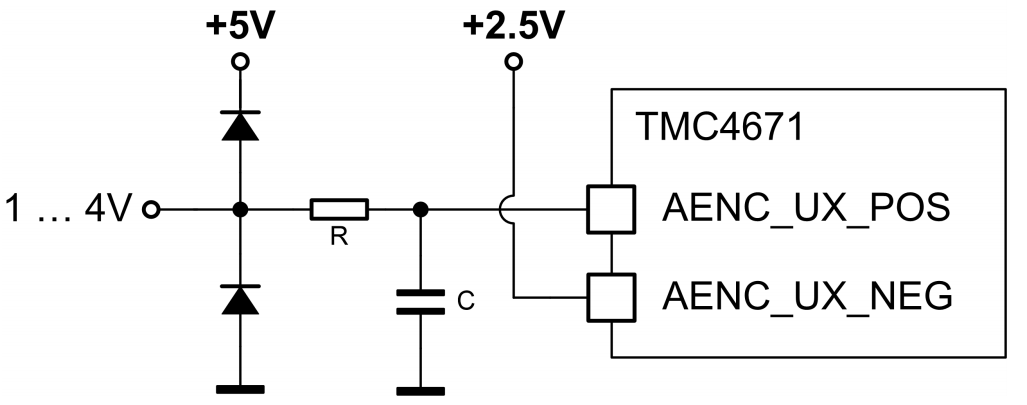
\includegraphics[width=0.5\textwidth]{graphics/Schema_Encoder_2_LP.png}
	\caption{Teilschema aus Datenblatt TMC4671. Hier mit Shottky-Dioden anstelle IC.}
	\label{fig:Schema_Encoder_2_LP}
\end{figure}

Die Widerstände \textbf{R703-R708} Stellen Spannungsteiler dar, welche gemäss Datenblatt eine benötigte Spannung von 2.5V bereitstellen.

Der Kondensator \textbf{C703} ist ein Stützkondensator und dient der Speisung eines Ecoders. Die Versorgungsspannung wird jedoch nicht für den Resolver benötigt.

Der Header \textbf{J6} ermöglicht, den Resolver an das PCB anzuschliessen.

Abbildung \ref{fig:Schema_Encoder_LP} zeigt das Gesamte Schema mit den Komponenten, welche ein korrektes Einlesen des Resolvers ermöglichen.

\begin{figure}[h!]
	\centering	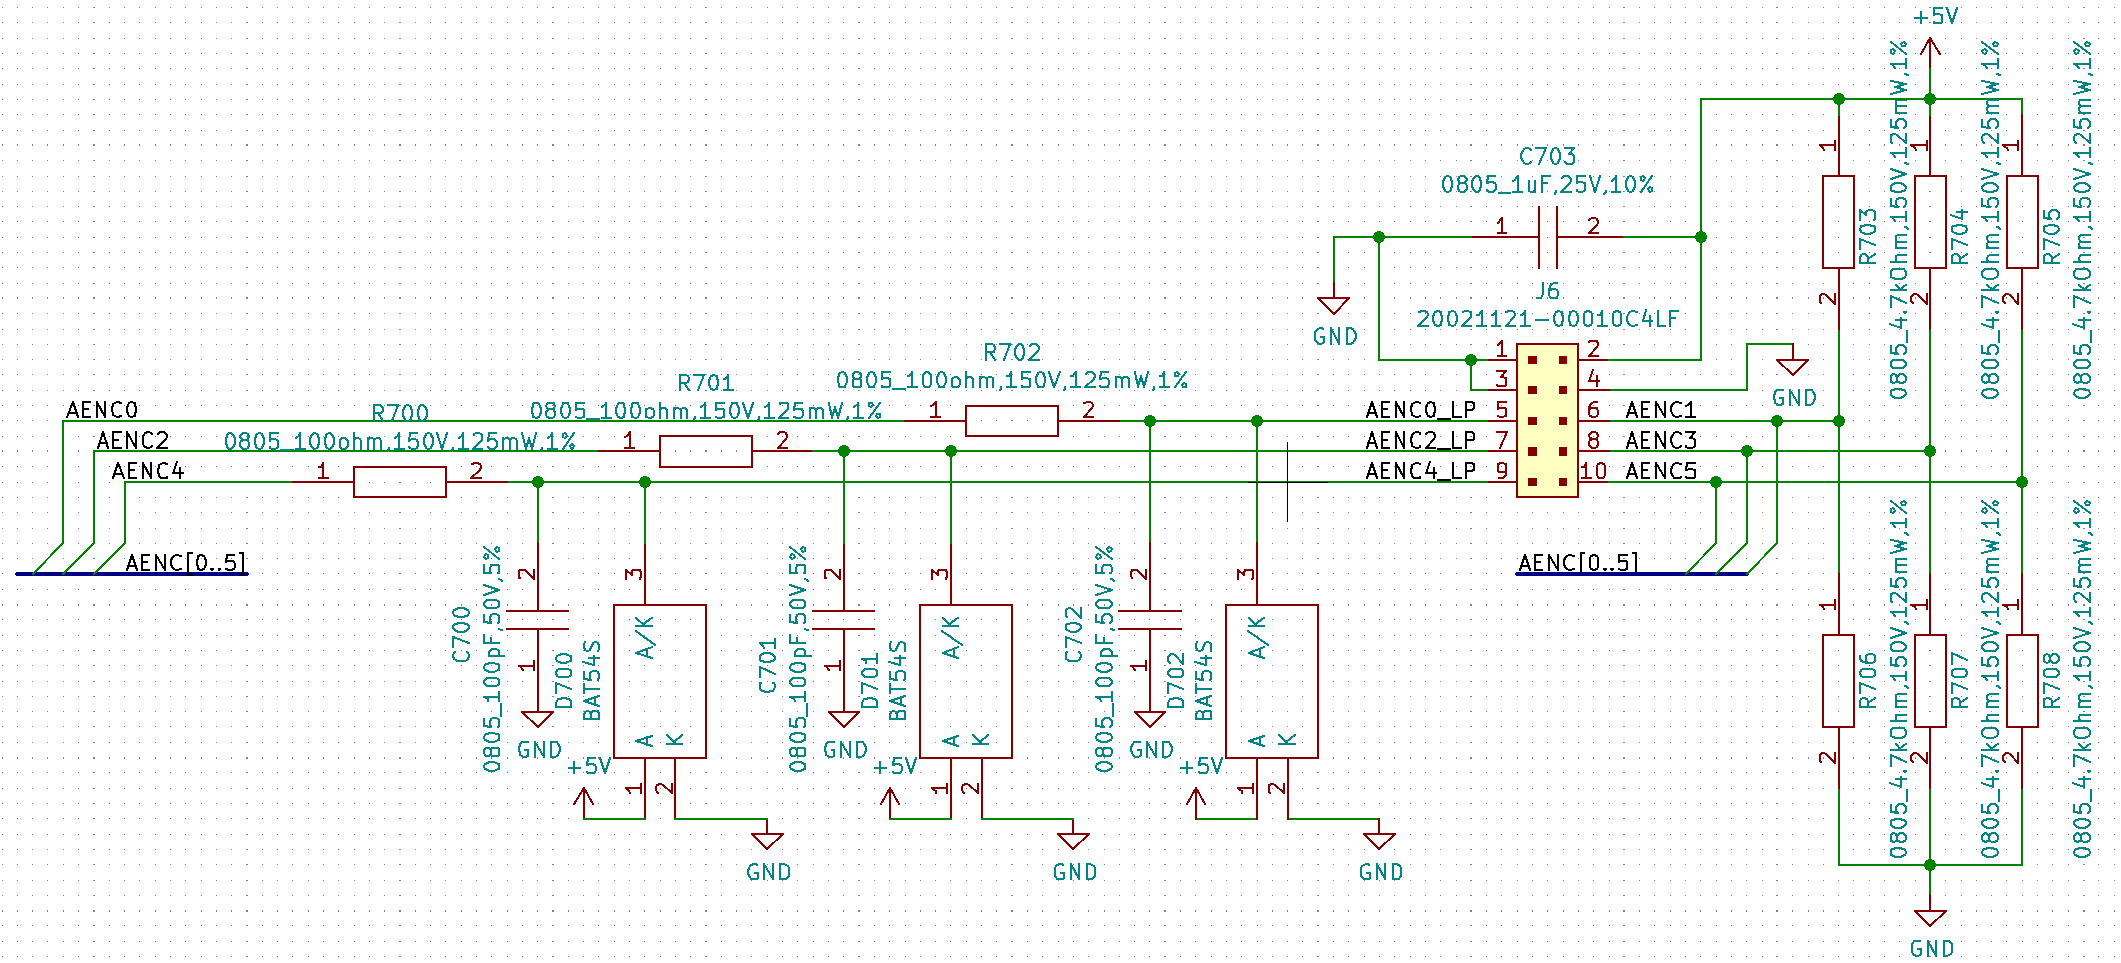
\includegraphics[width=\textwidth]{graphics/Schema_Encoder_LP.png}
	\caption{Teilschema TMC4671. Hier Input Encoder.}
	\label{fig:Schema_Encoder_LP}
\end{figure}
\newpage
\subsubsection{Analog-Inputs}\label{subsubsec:Analog_Inputs}

Auch hier wird das Eingangssignal mit einem Tiefpass gefiltert. Dafür werden die Widerstände R711 und R713 sowie die Kondensatoren C707 und C709 verwendet. Die Beschaltung und Dimensionierung wurde aus dem Datenblatt des TMC4671-EVAL-Board entnommen. Die Zeitkonstante des Filters beträgt gemäss Formel \ref{equ:Berechnung_Analog_LP} 400ns. Das Schaltungsprinzip ist in Abbildung \ref{fig:Schema_Analog_LP} dargestellt. \cite[PDF S.25]{trinamic_drawings_2018}
\begin{equation}
\tau = R \cdot C = 4\cdot 10^{3}\Omega \cdot 100\cdot10^{-12}F = 10 \cdot 10^{-9}s = 400ns
\label{equ:Berechnung_Analog_LP}
\end{equation}

Weiter befindet sich ein zweiter Widerstand in jeder Schaltung
\todo{Funktion zweiter Widerstand herausfinden.}

Das letzte Bauteil, welches noch beschrieben werden muss, sind die Dioden D703 und D704. Diese stellen jeweils wieder einen Über- bzw. Unterspannungsschutz dar, um den Messeingang des TMC4671 zu schützen. Das Bauteil ist das selbe wie oben im Encoder-Teil, weshalb hier auf eine tiefere Beschreibung verzichtet wird.

\begin{figure}[h!]
	\centering	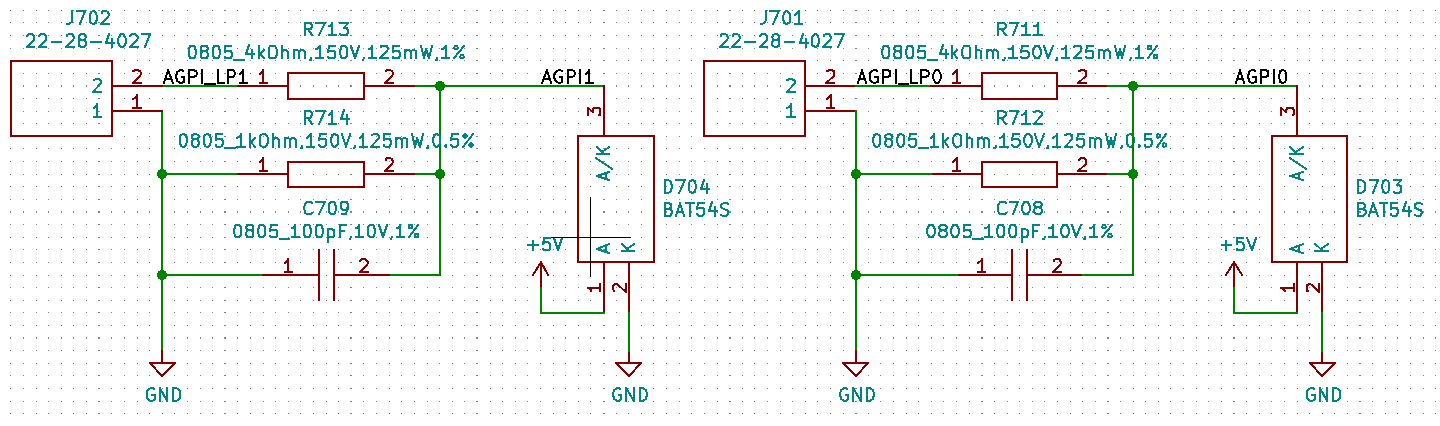
\includegraphics[width=0.8\textwidth]{graphics/Schema_Analog_Inputs_LP.png}
	\caption{Teilschema TMC4671. Hier Inputs Analog.}
	\label{fig:Schema_Analog_LP}
\end{figure}

\newpage

\subsubsection{Motorspannung-Input}\label{subsubsec:Motorspannung_Input}

\cite[PDF S.25]{trinamic_drawings_2018}
\begin{figure}[h!]
	\centering	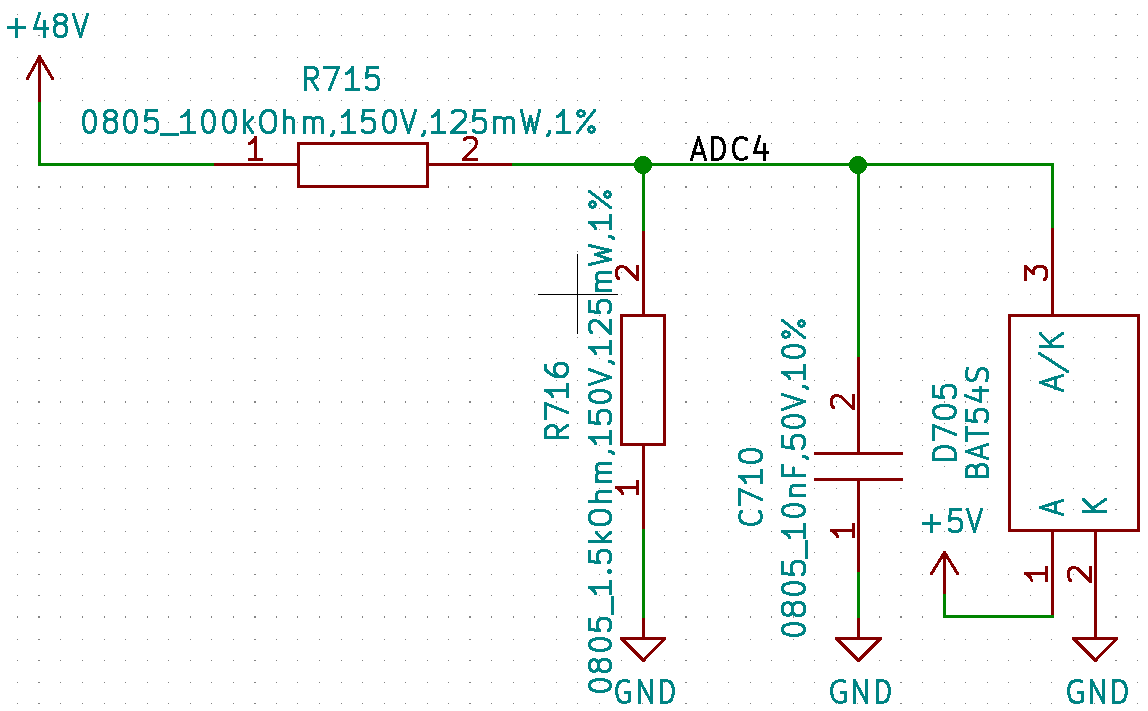
\includegraphics[width=0.45\textwidth]{graphics/Schema_VM_Input_LP.png}
	\caption{Teilschema TMC4671. Hier Input Motorspannung.}
	\label{fig:Schema_Encoder_LP}
\end{figure}

\newpage

\subsubsection{Temperatur-Input}\label{subsubsec:Temperatur_Input}

\cite[PDF Schematic S.3]{trinamic_tmc-ups-10a70v--eval_nodate}
\begin{figure}[h!]
	\centering	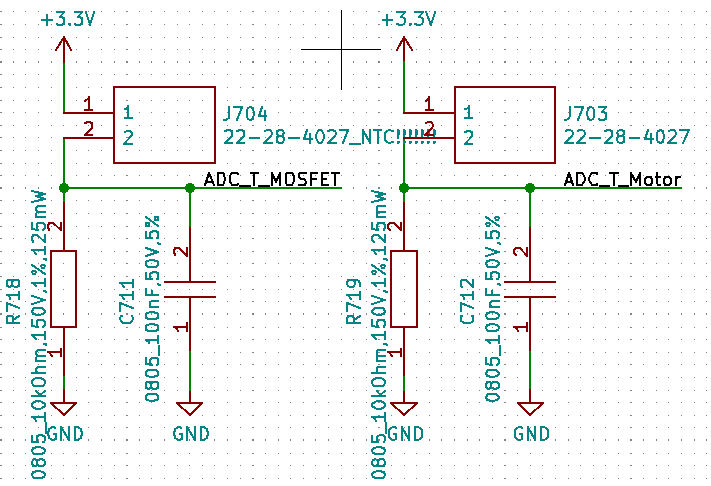
\includegraphics[width=0.45\textwidth]{graphics/Schema_Temperaturen_LP.png}
	\caption{Teilschema TMC4671. Hier Input Temperaturen.}
	\label{fig:Schema_Encoder_LP}
\end{figure}